Before we started coding we made a draft of the class diagrams. Throughout the following sprints we kept maintaining and updating the class diagram
draft to make sure that the code and class diagram were in agreement. The class diagram shown and explained below is the final version for our
system.

The class diagram is made in the Unified Modeling Language (UML) to ensure common understanding, when describing the structure of our system.

\begin{figure}[htb]
    \begin{center}
        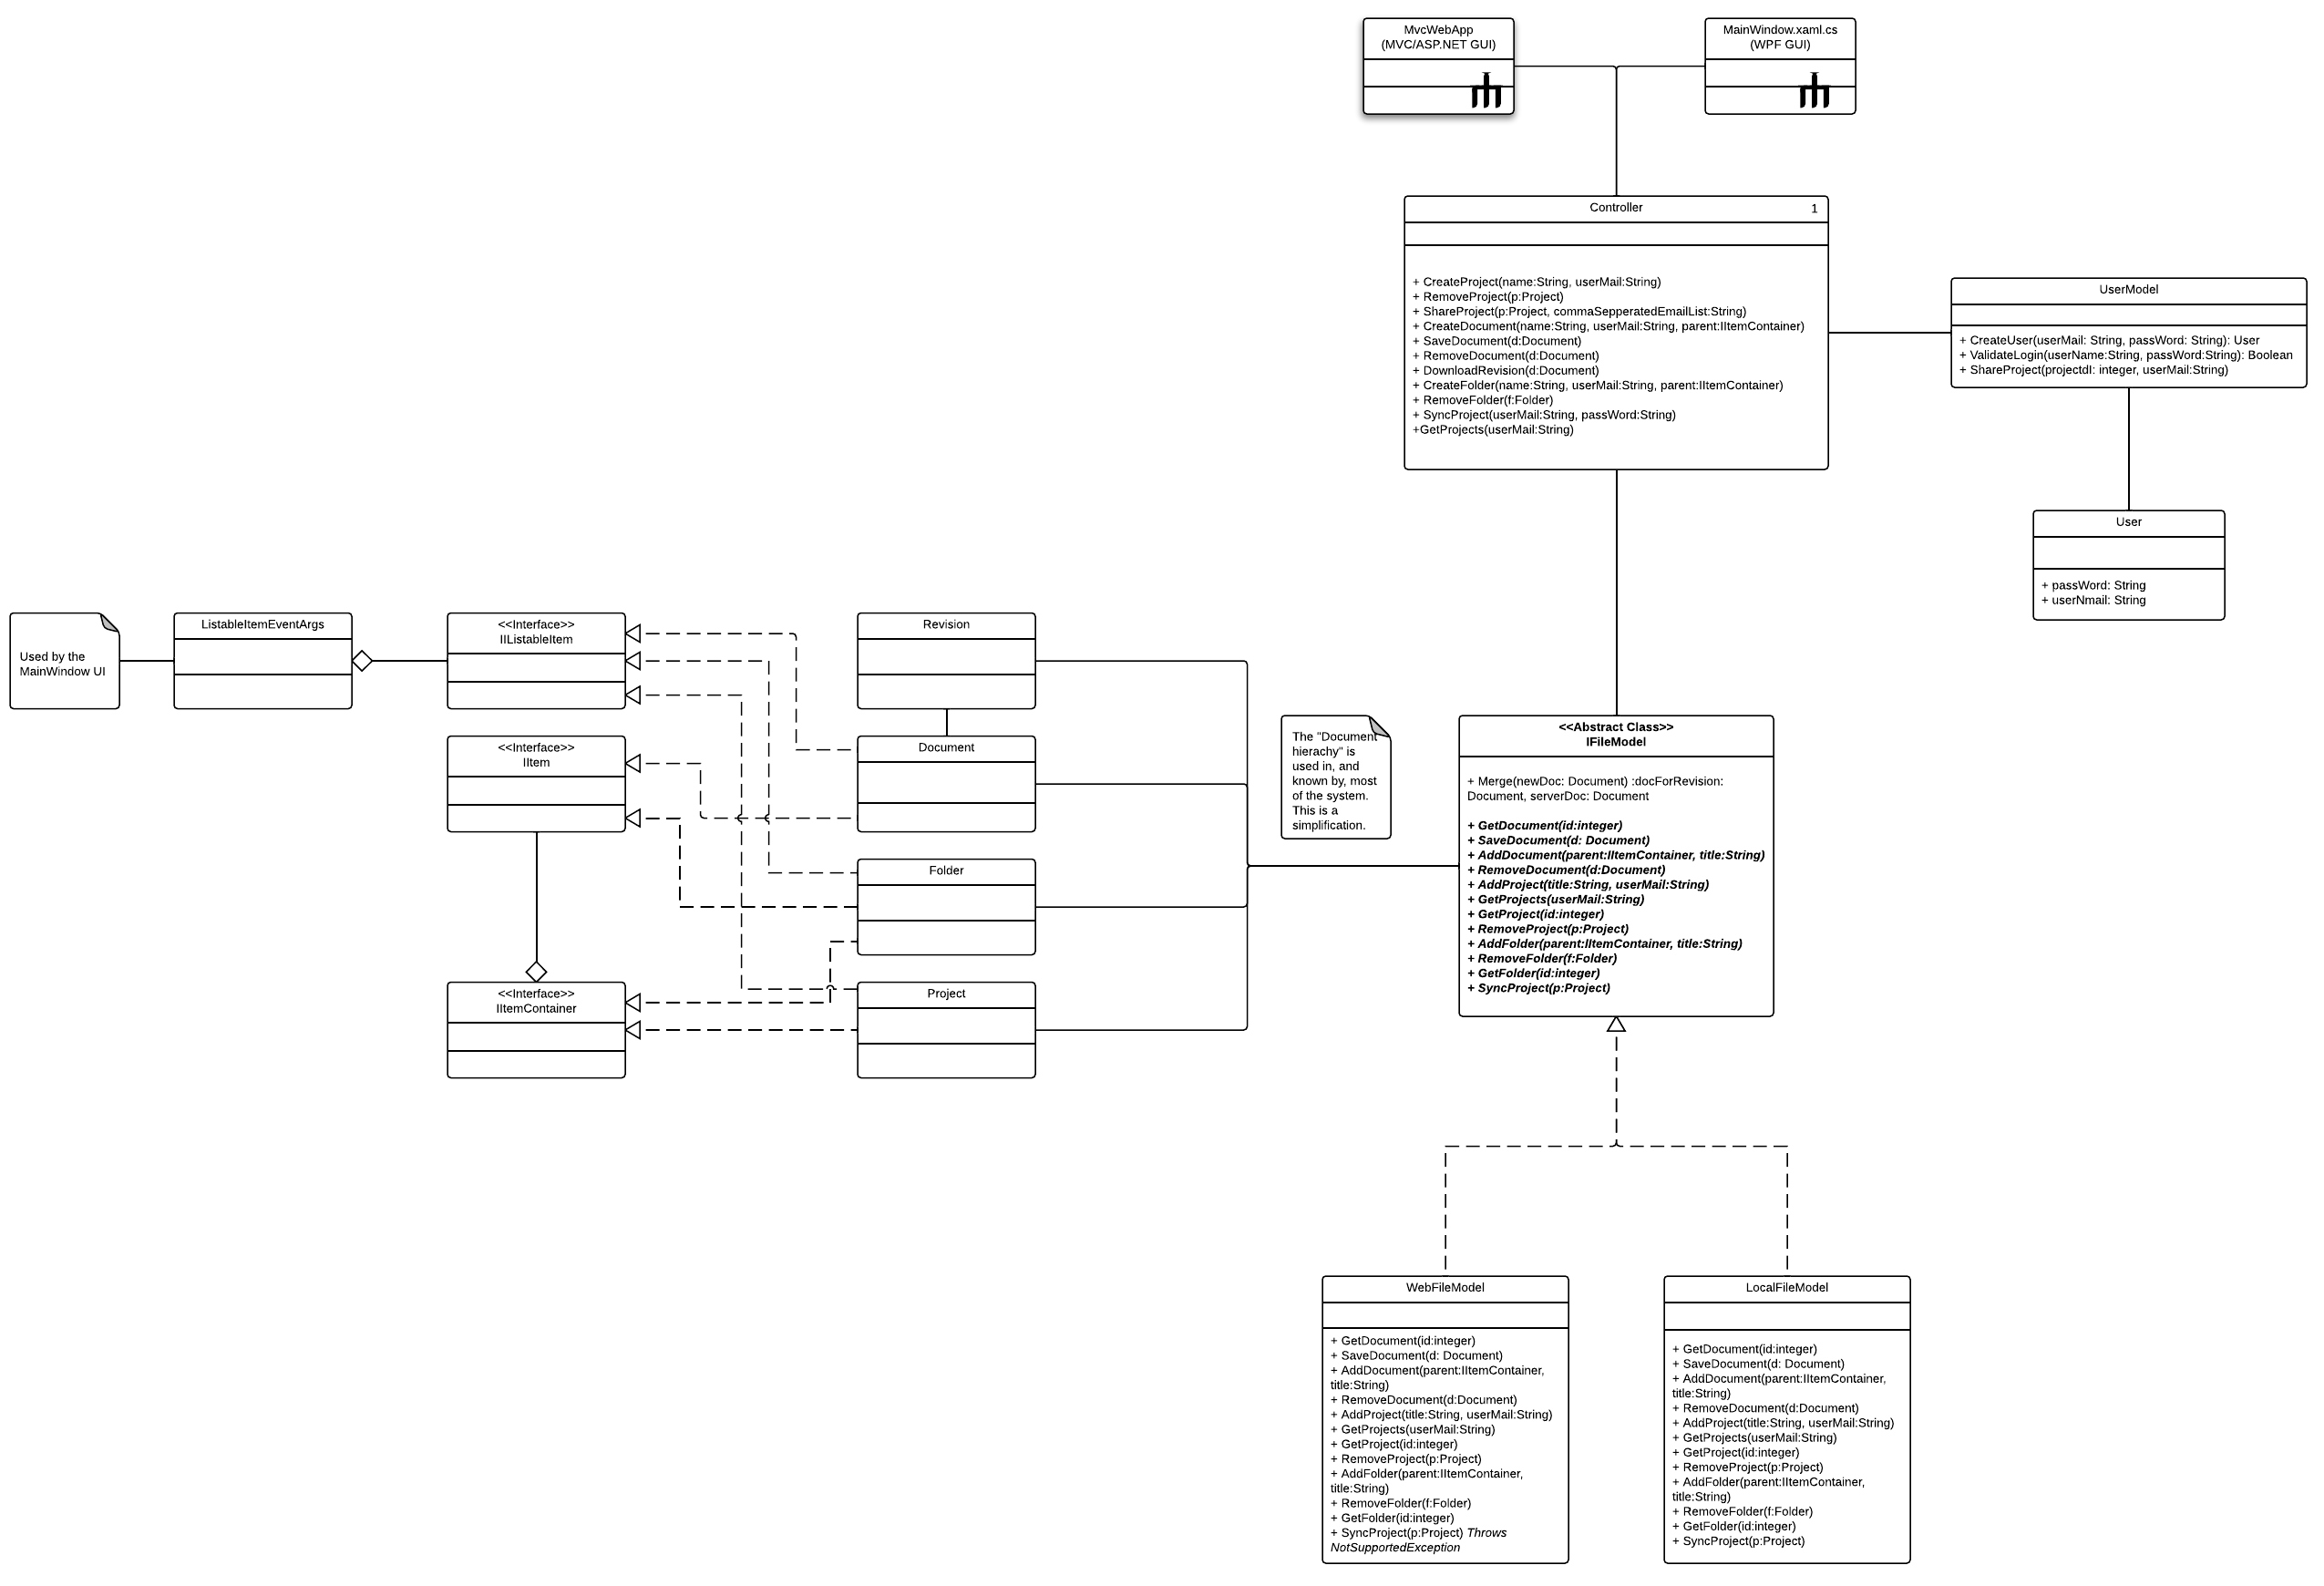
\includegraphics[width=1\textwidth]{Software_design/graphics/mainClassDiagram.png}
        \caption{Overview of the simplified main class diagram for 'Slice of Pie'}
        \label{fig:design-class_diagram}
    \end{center}
\end{figure}

In (Figure~\ref{fig:design-class_diagram}) the most critical and important classes are shown with their most important attributes and public methods.
None of the two GUIs (MvcWebApp and MainWindow) are shown in the class diagram, but are in two separate class diagrams. This is shown with the rake
symbol on the two classes in the main class diagram.

%Fill in some explanation about the diagram

\subsubsection{The MvcWebApp GUI}

This diagram can be found in the (Appendix~\ref{fig:mvcwebapp-diagram})
